\documentclass[a4paper]{article}

\usepackage[english]{babel}
\usepackage[utf8]{inputenc}
\usepackage{amsmath}
\usepackage{graphicx}
\usepackage[colorinlistoftodos]{todonotes}
\usepackage{listings}
\usepackage{float}
\renewcommand{\floatpagefraction}{.8}%
\title{Singular value decomposition}

\author{Vladislav Iliushin}

\date{\today}

\begin{document}
\maketitle

 

\section{Approximation}

\subsection{Total least squares approximation}
 
 
\begin{figure}[h]
	       
	       	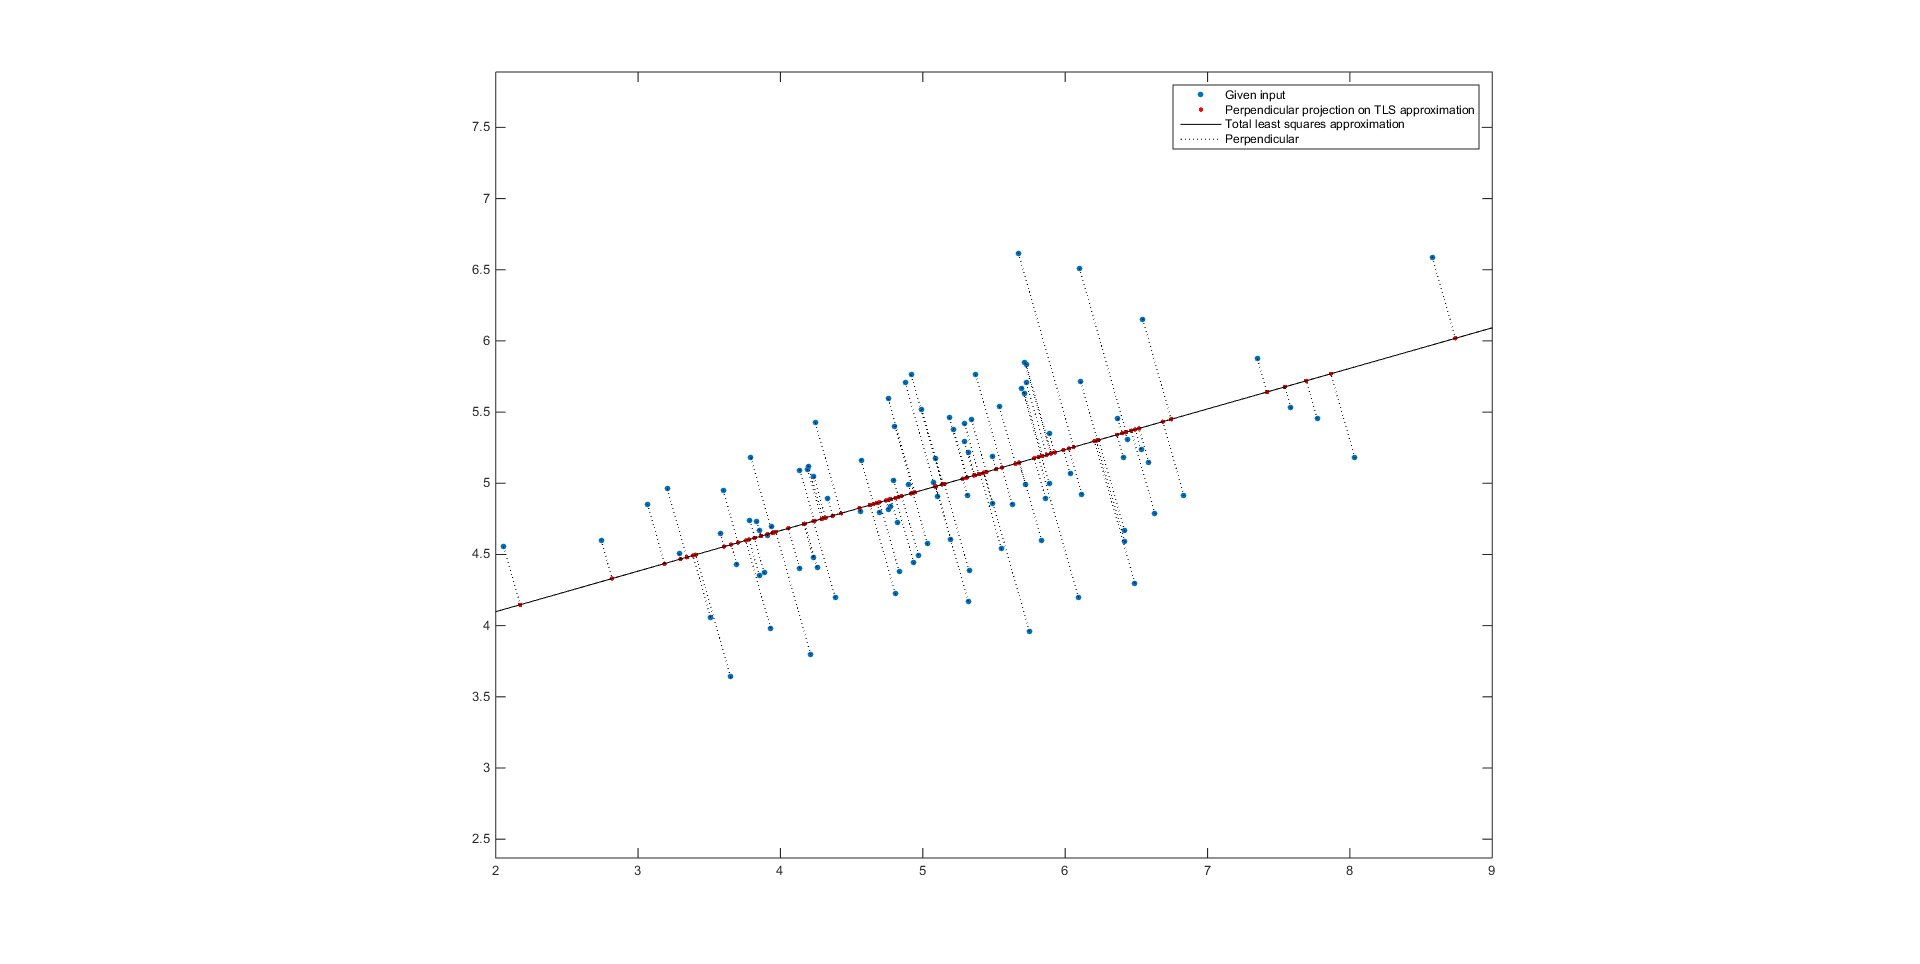
\includegraphics [width=1.2\textwidth] {part1/TLS.png}
	       	\caption{Total least squares approximation}
	\label{fig:TLS}
      

\end{figure}
\
\subsection{Perpendicular squares sum}

\[ \textup{d}(\mathbf{p,q})=  \sqrt[2]{(p_{1} - q_{1}) ^{2} + (p_{2} - q_{2})^{2}}  \]
\\
For given points and considering that square area is equal to $\textup{d}(p,q)^{2}$ we get 
\\
\[ \sum \textup{d}(\mathbf{p_,q})^{2} =  \sum_{i=1}^{n} d(p_{i}, q_{i})^{2} = 24.2419 \]

Matlab code:
\begin{lstlisting}
 error = norm(A_approx-A).^2;
 \end{lstlisting}
 
 \subsection{Different representations}
 
 \[ \mathbf{x}= \{ v_{2,1}, v_{2,2} \} \]
 Matlab code:
 \begin{lstlisting}
  x = V(2,:);
 \end{lstlisting}
  \[ \alpha = v_{2,1}  \cdot  \bar{x} +v_{2,2} \cdot \bar{y}  \]
   Matlab code:
   \begin{lstlisting}
  l1=V(2,1);
  l2=V(2,2);
  alpha=l1*xMean(1)+l2*xMean(2);
  \end{lstlisting}
 \[ \mathbf{y_{0}} = A_{approximation}(0,0) \]
    Matlab code:
  \begin{lstlisting}
A = [0 0 ;A];
... approximation code ...
y0 = A_approx(1,:);
  \end{lstlisting}
  \[\mathbf{s} = \{v_{1,1}, v_{1,2} \}\]
  Matlab code:
    \begin{lstlisting}
  s = V(1,:);
    \end{lstlisting}
\section{Motion capture sequence compression}

\subsection{Squares sum minimization}

\begin{table}[h]
	\begin{tabular}{ll}
		"R" rank & Optimal value \\
		 \hline 
		1        & $4.6166 \cdot 10^{8} $      \\
		 \hline 
		2        & $1.6925 \cdot 10^{8} $      \\
		 \hline 
		5        & $1.0453 \cdot 10^{7} $      \\
		 \hline 
		10       & $1.1982 \cdot 10^{6} $      \\
		 \hline 
		15       & $2.5626 \cdot 10^{5} $      
	\end{tabular}
\end{table}
\
\subsection{Linear combination of span vector}

\begin{figure}[h!]
	\centering
	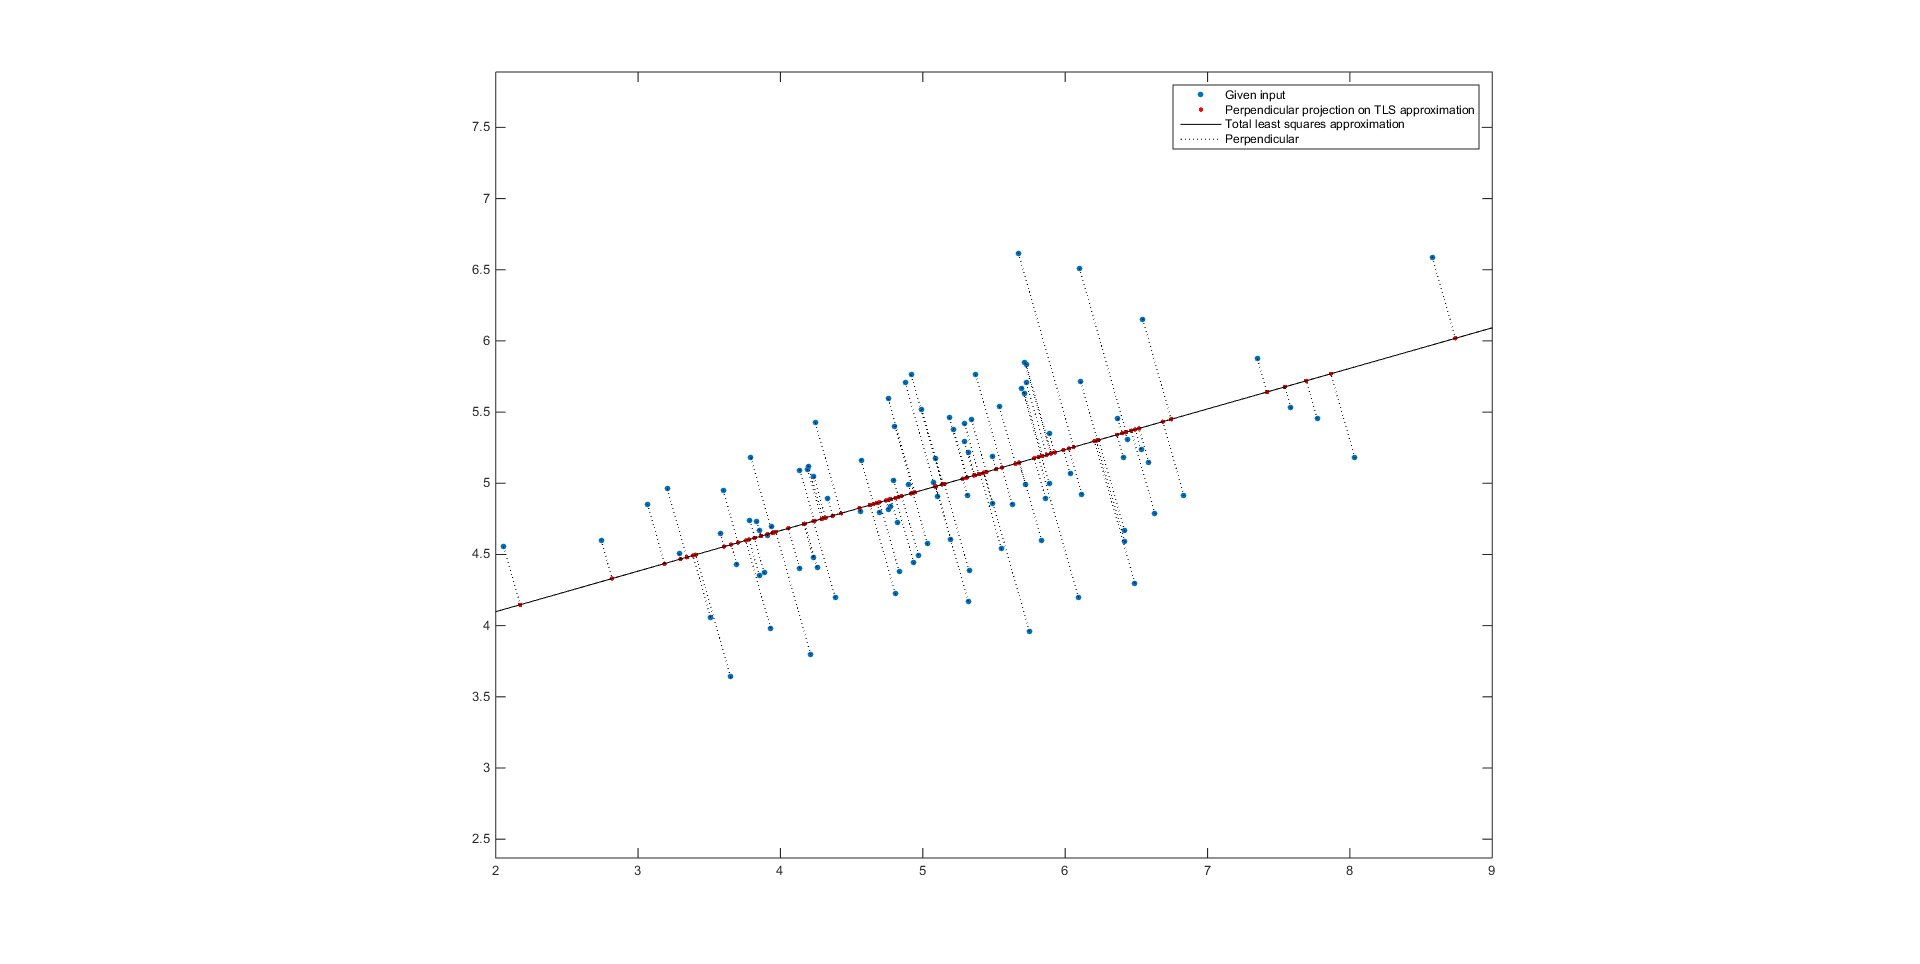
\includegraphics [width=0.8\textwidth] {part1/TLS.png}
	\caption{Total least squares approximation}
	\label{fig:2d1}
	
	
\end{figure}

\begin{figure}[h!]
	\centering
	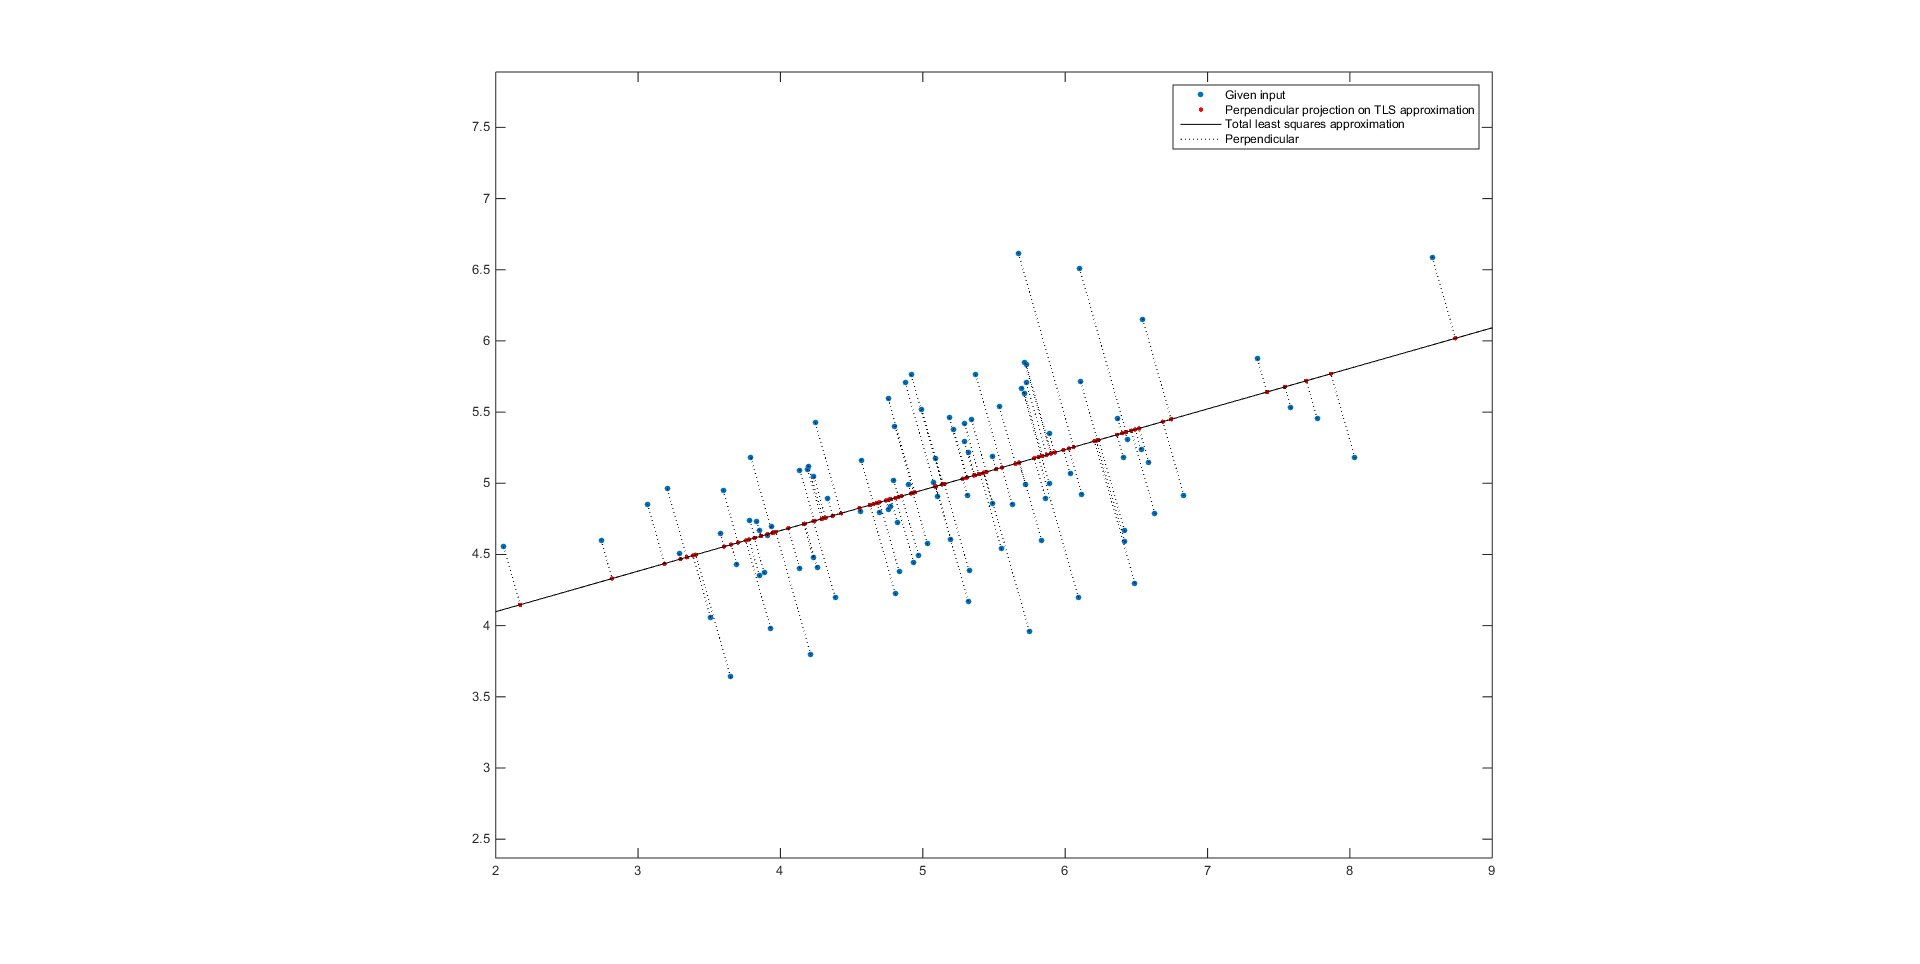
\includegraphics [width=0.8\textwidth] {part1/TLS.png}
	\caption{Total least squares approximation}
	\label{fig:2d2}
	
	
\end{figure}

\begin{figure}[h!]
	\centering
	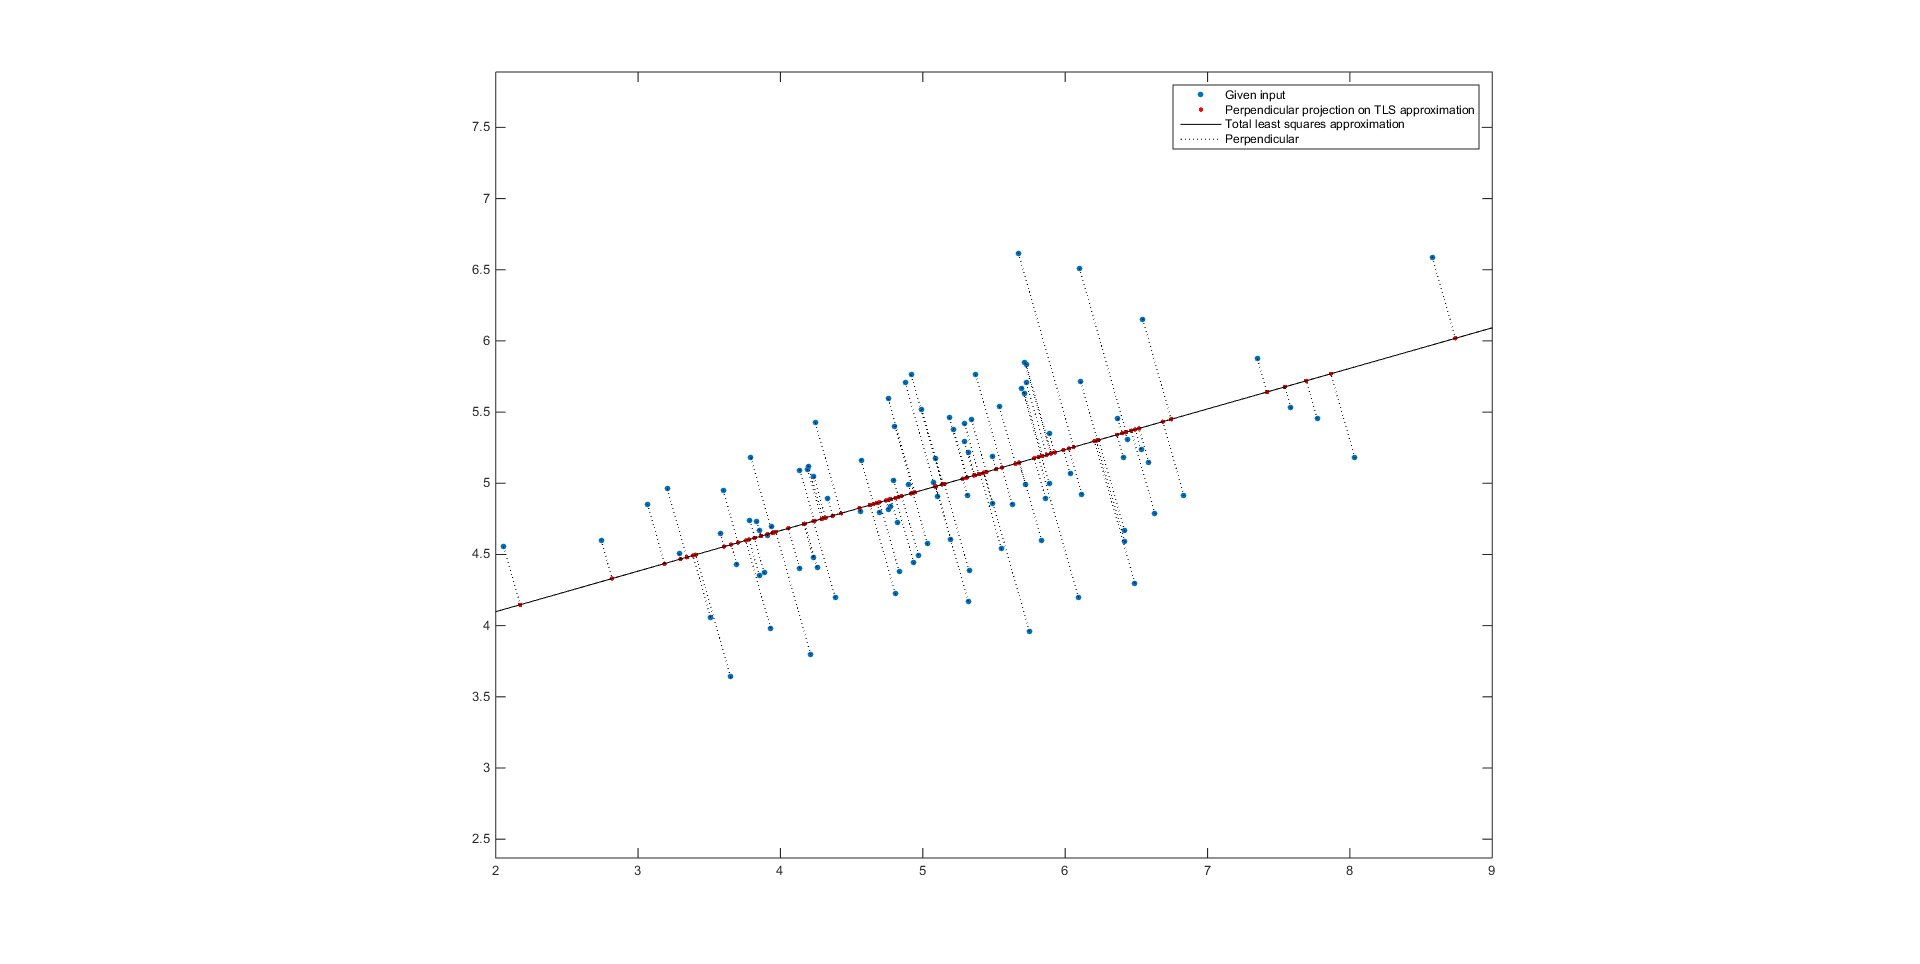
\includegraphics [width=0.8\textwidth] {part1/TLS.png}
	\caption{Total least squares approximation}
	\label{fig:3d1}
	
	
\end{figure}

\begin{figure}[h!]
	\centering
	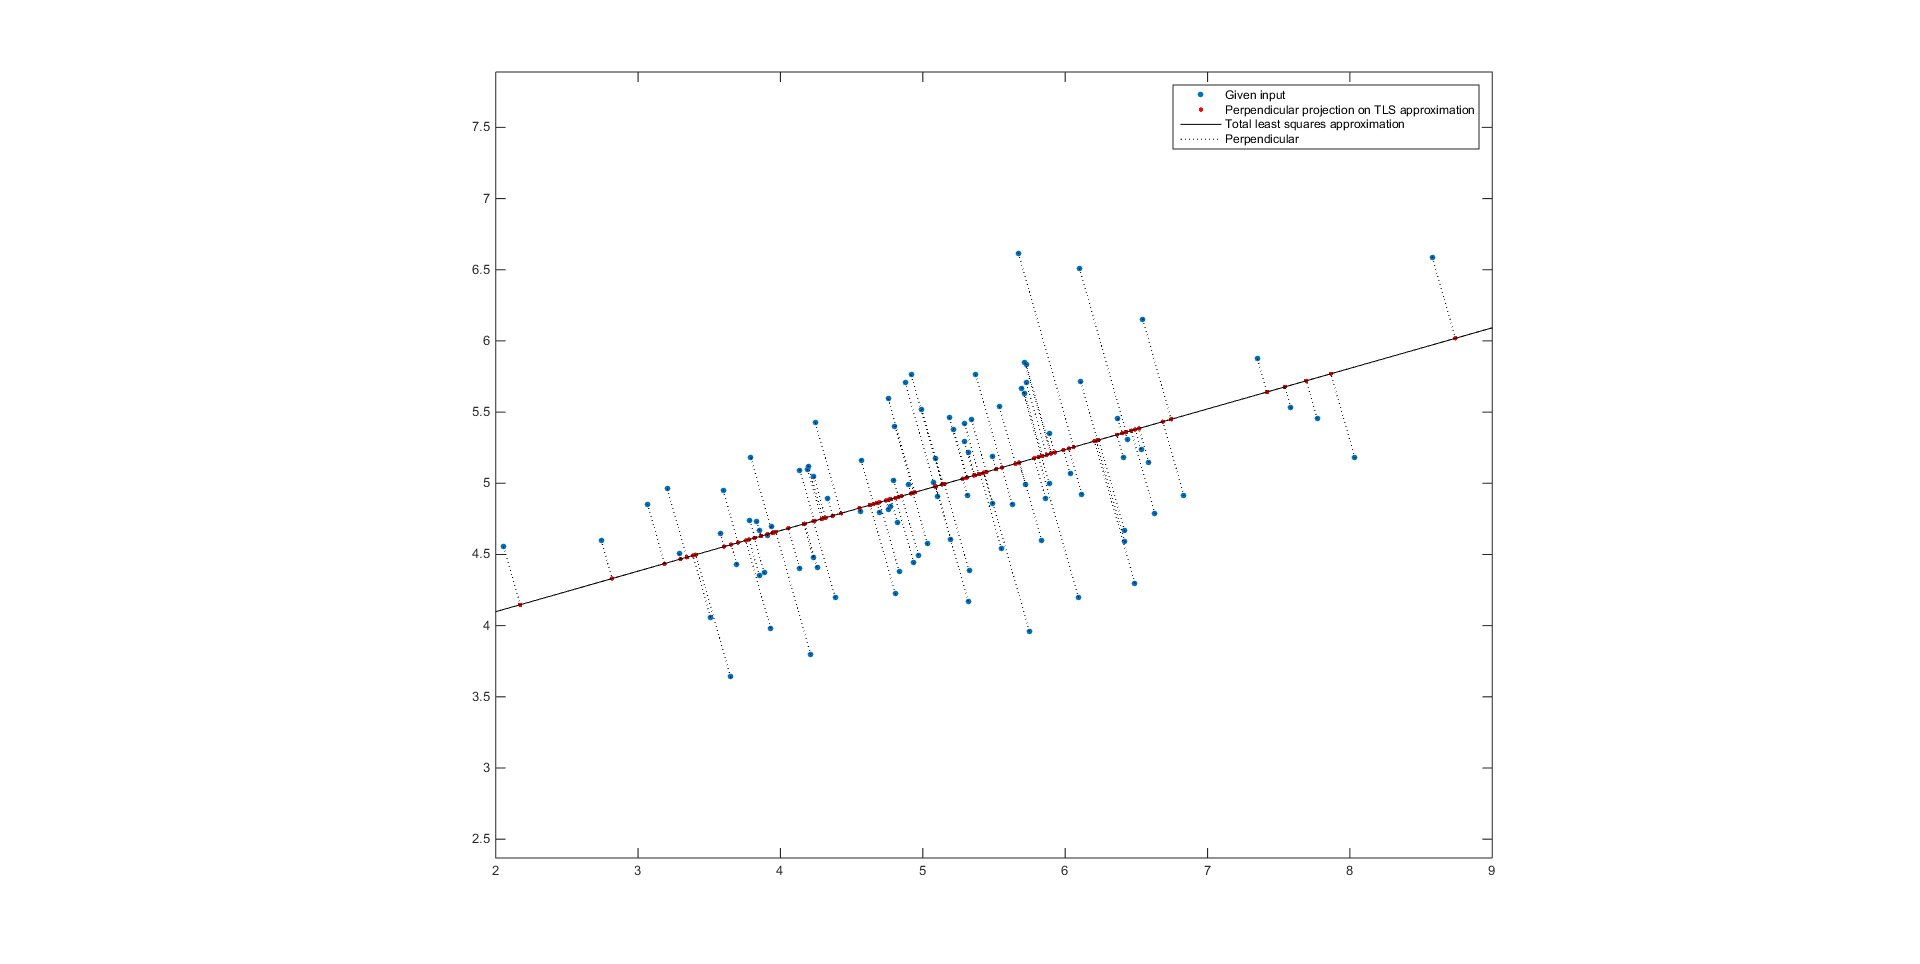
\includegraphics [width=0.80\textwidth] {part1/TLS.png}
	\caption{Total least squares approximation}
	\label{fig:3d2}
	
	
\end{figure}
\
\subsection{Minimization of approximation data dimension}

\subsection{Approximation optimal error}

 

\end{document}\documentclass[10pt]{•}